\section{Calcolo delle portate di progetto (analisi dei deflussi di piena)}
Al fine di conoscere la quantità di deflusso prevista alla sezione di chiusura, occorre prima ricavarsi dei parametri fisici del bacino.

\subsection{Calcolo del tempo di corrivazione del bacino}
Il tempo di corrivazione di un bacino è il tempo che impiega una particella d'acqua ad arrivare alla sezione di chiusura, partendo dal punto idraulicamente più distante da essa.\\
La conoscenza del tempo di corrivazione del bacino permette di prevedere il momento in cui avviene il picco di deflusso alla sezione di chiusura.\\
Esistono diverse metodologie per calcolare il tempo di corrivazione del bacino: metodo cinematico, metodo empirico di Giandotti, di Ferro,...
\subsubsection{Metodo cinematico}
Il metodo cinematico per il calcolo del tempo di corrivazione del bacino implica lo studio del moto dell'acqua sia nel tratto di versante e sia nel tratto di reticolo idrografico.
\begin{equation}
    T_c = T_v + T_r
    \label{tempo_corrivazione}
\end{equation}
Dove:
\begin{itemize}
    \item $T_c$: tempo di corrivazione;
    \item $T_v$: tempo di versante;
    \item $T_r$: tempo di reticolo.
\end{itemize}
Sia per il calcolo del movimento dell'acqua nel reticolo e sia per quello nel versante, è necessario conoscere alcune quote altimetriche del bacino:
\begin{itemize}
    \item $h_0$ (quota della sezione di chiusura): 1183 m s.l.m.;
    \item $h_r$ (quota superiore del collettore principale): 1883 m s.l.m.;
    \item $h_s$ (quota massima del bacino): 2084.3 m s.l.m. 
\end{itemize}
Partendo dalla formula generale della velocità di un fluido: 
\begin{equation}
    V = K_s \cdot R_h^{\frac{2}{3}} \cdot i ^{\frac{1}{2}}
\end{equation}
e svolgendo alcune semplificazioni, è possibile ottenere le formule per il calcolo della velocità nel reticolo e nel versante:
\begin{equation}
    V_R \approx (5 - 10) \cdot i^{\frac{1}{2}}
    \label{vel_reticolo}
\end{equation}
\begin{equation}
    V_v \approx (0.1 - 0.15) i_v^{\frac{1}{2}}
    \label{vel_versante}
\end{equation}
La formula del tempo di corrivazione \ref{tempo_corrivazione} può essere implementata con le formule \ref{vel_versante} e \ref{vel_reticolo}:
\begin{equation}
    T_c = \frac{L_R}{V_R}+ \frac{L_V}{V_V} \approx \frac{L_R}{(5 - 10) \cdot i^{\frac{1}{2}}} + \frac{L_V}{(0.1 - 0.15) i_v^{\frac{1}{2}}}
\end{equation}

Per il calcolo della velocità di reticolo dell'acqua nel bacino, è necessario imporre un valore di pendenza del retico; questo valore si ricava dal rapporto tra la differenza di quota del collettore principale (1883 m-1183 m) e la sua lunghezza (2401 m).\\
Svolgendo la formula \ref{vel_reticolo}, imponendo un coefficiente medio di 7.5, il risultato è $4.05 \frac{m}{s}$.\\
Conoscendo la lunghezza del collettore principale, è possibile ricavare il tempo di corrivazione della componente del reticolo idrografico.\\
In modo analogo, il calcolo della velocità dell'acqua nel versante avviene conoscendo la pendenza del tratto di terreno, ovvero il rapporto tra la differenza di quota (2084.3 m-1883 m) e la sua distanza, ricavata dal GIS, di 445.16 m.\\
Applicando la formula \ref{vel_versante}, applicando un coefficiente di 0.15, la velocità di versante risulta essere di $0.10 \frac{m}{s}$.\\
Anche in questo caso, il tempo di corrivazione nel versante è ricavabile invertendo la formula della velocità.
I tempi di percorrenza dell'acqua sono:
\begin{table}[H] \centering
    \begin{tabular}{ccc}
        \toprule
    \textbf{$T_v$} & \textbf{$T_r$} & {\color[HTML]{000000} } \\
    4413.28     & 592.90      & sec                     \\
    1.23        & 0.16        & ore       \\
    \bottomrule             
    \end{tabular}
    \end{table}
Il tempo di corrivazione totale, ovvero la somma dei due parziali, risulta essere pari a 83.44 minuti (ovvero 1.39 ore).

\subsubsection{Metodo empirico di Giandotti}
Il metodo di Giandotti, per il calcolo del tempo di corrivazione del bacino, richiede l'applicazione della relativa formula:
\begin{equation}
    T_c = \frac{4 \cdot \sqrt{A}+ 1.5 \cdot L}{0.8 \cdot \sqrt{H_m}}
\label{formula_giandotti}
\end{equation}
Dove: 
\begin{itemize}
    \item $T_c$: è il tempo di corrivazione, espresso in ore;
    \item A: è l'area del bacino, espressa in $km^2$;
    \item L: è lunghezza del collettore idraulico, estesa fino allo spartiacque, espressa in km;
    \item $H_m$: è l'altezza media del bacino, riferita alla sezione di chiusura ed espressa in m.
\end{itemize}
Per il bacino in esame:
\begin{itemize}
    \item A: 2.01 $km^2$;
    \item $L_c$: 2.846 $km$;
    \item $H_m$: 470.9 $m$.
\end{itemize}
La formula di Giandotti \ref{formula_giandotti}, con i parametri del bacino in esame, restituisce il tempo di corrivazione di 34.4 minuti (0.573 ore).\\
Questa formula notoriamente restituisce valori di corrivazione molto contenuti rispetto a quelli reali.

\subsubsection{Metodo empirico di Ferro (I)}
La formula necessaria da applicare per questo metodo è la seguente:
\begin{equation}
    T_c = 0.022 \cdot \left(\frac{L_C}{i^{0.5}}\right)^{0.8}
    \label{formula_ferro_I}
\end{equation}
Dove: 
\begin{itemize}
    \item $T_c$: viene espressa in minuti;
    \item $L_C$: viene espressa in metri;
    \item i: viene espressa $\frac{m}{m}$.
\end{itemize}
Nel caso del bacino in esame:
\begin{itemize}
    \item A: 2.01 $km^2$;
    \item $L_C$: 2401 $m$;
    \item $i_r$: 0.293 $\frac{m}{m}$.
\end{itemize}
La formula del metodo di Ferro (I) \ref{formula_ferro_I} restituisce il valore di 18.19 minuti.\\
Nel caso di bacini montani con collettore principale corto (qualche chilometro), e ripido, la formula tende a sottostimare il valore reale.

\subsubsection{Metodo empirico di Ferro (II)}
La formula di Ferro (II) richiede solamente la conoscenza dell'area del bacino:
\begin{equation}
    T_c = 0.675 \cdot \sqrt{A}
    \label{formula_ferro_II}
\end{equation}
Dove:
\begin{itemize}
    \item $T_c$: viene espressa in ore;
    \item $A$: viene espressa in $km^2$.
\end{itemize}
Nel caso del nostro bacino, come già riportato prima, l'area è pari a 2.01 $km^2$.\\
La formula \ref{formula_ferro_II} restituisce un tempo di corrivazione pari a 57.42 minuti (0.96 ore).

\subsection{Comparazione dei metodi di corrivazione}
Dopo aver applicato diversi metodi per il calcolo del tempo di corrivazione, risulta utile compararli.
\begin{table}[H] \centering
    \caption{\textcolor{red}{Comparazione dei diversi metodi di calcolo del tempo di corrivazione.}}
    \begin{tabular}{ccc}
        \toprule
  Metodo di calcolo   & $T_c$ in minuti & $T_c$ in ore\\
     \midrule
   Cinematico  & 83.44 & 1.39\\
   Giandotti  & 34.356 & 0.573\\
   Ferro (I)  & 18.19 & 0.30\\
   Ferro (II)  &57.42 & 0.96\\
     \bottomrule
    \end{tabular}
    \end{table}
A seconda del caso di studio o di lavoro in esame, ogni metodo di calcolo trova la propria migliore applicazione.\\
Ovviamente, conoscendo le distanze dei tratti (di reticolo e di versante) e le relative velocità dell'acqua in movimento, il metodo cinematico risulta quello che calcola nel modo più affidabile possibile il tempo di corrivazione del bacino. Lo stesso ragionamento può essere svolto considerando che tale metodo è l'unico fisicamente basato tra tutti quelli elencati. Per tali motivi, verrà utilizzato questo risultato per le successive valutazioni inerenti ai calcoli dei deflussi attesi.\\
Nei casi in cui, per questioni di tempo o per mancanza di dati, il metodo cinematico non fosse utilizzabile, l'applicazione degli altri metodi per il calcolo del tempo di corrivazione dev'essere svolta considerando l'assunzione di inevitabili errori. 

\subsection{Determinazione del parametro idrologico CN}
Al fine di descrivere la tendenza di un suolo a generare runoff o infiltrazione sottosuperficiale (a fronte di un evento pluviometrico), il dipartimento di agricoltura americano (USDA) ha idealizzato il metodo SCS-CN (\textit{soil conservation service - curve number}).\\
In seguito ad analisi empiriche, ad ogni tipologia di suolo e soprassuolo sono associati precisi valori, in una scala che va da 0 a 100.\\
Maggiore è il valore attribuito all'area e maggiore è la tendenza che si crei deflusso superficiale. Viceversa, minore è il numero dell'indice e maggiore sarà la capacità del suolo ad infiltrare acqua. I valori CN sono generalmente tabellati, e rilasciati da vari enti pubblici (\ref{scs_cn_table}).\\
La qualità litologica del suolo viene descritta secondo 4 gruppi (dalla A alla D), con capacità di infiltrazione dell'acqua sempre minore.\\

\begin{figure}[H]  \centering
    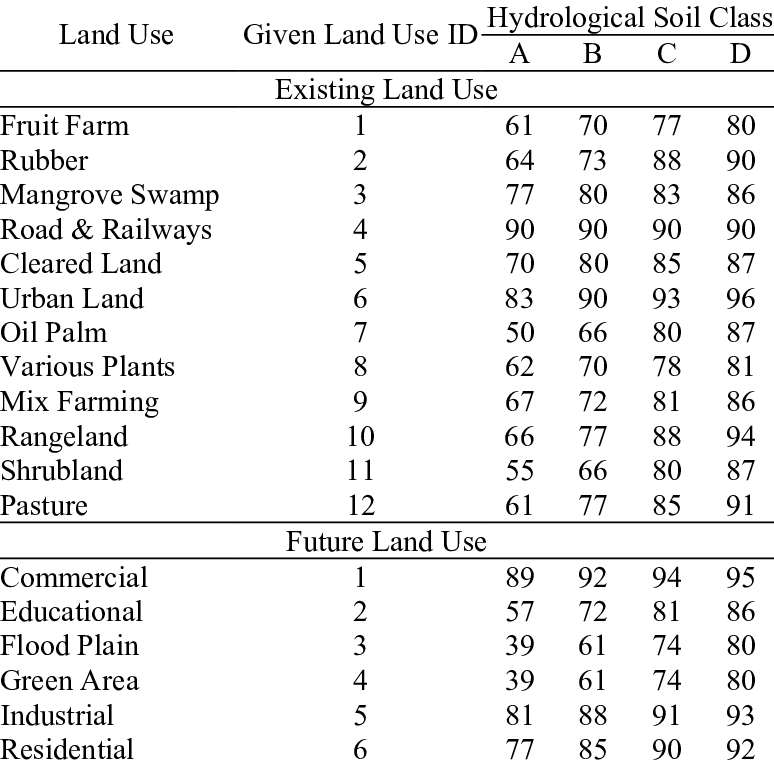
\includegraphics[scale=0.5]{immagini/scs_cn_table.png}
    \caption{Valori tabellari del parametro idrologico CN.}
    \label{scs_cn_table}
\end{figure}

Il parametro CN, oltre che essere dipendente dalla natura del suolo o dall'utilizzo del soprassuolo, viene influenzato anche dalle condizioni pluviometriche incidenti nei giorni precedenti del momento di studio.\\
Generalmente, tutti i valori tabellati, a meno che non venga specificato, si trovano in condizione AMC (\textit{Antecedent Moisture Conditions}) numero II, ovvero in grado medio.\\
I parametri AMC vengono imposti considerando le seguenti condizioni:
\begin{figure}[H]  \centering
    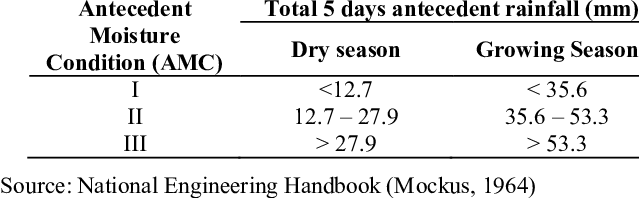
\includegraphics[scale=0.7]{immagini/AMC_table.png}
    \caption{Condizioni idrologiche del suolo antecedenti l'evento di pioggia AMC (I), AMC (II) e AMC (III).}
    \label{AMC_table}
\end{figure}
Le trasformazioni tra le diverse condizioni avvengono mediante le formule:
\begin{equation}
    AMC (I)\rightarrow CN (I) = \frac{4.2 \cdot CN(II)}{10-0.058 \cdot CN(II)}
\end{equation}
\begin{equation}
    AMC(III) \rightarrow CN(III) = \frac{23\cdot CN (II)}{10+0.13 \cdot CN(II)}
    \label{amcIII}
\end{equation}
La condizione più favorevole, ovvero la AMC (III), è quella che genera il maggior deflusso, e che è quindi preferibile da utilizzare in sede di progetto.\\
Il limite di saturazione dell'acqua nel terreno (S), ovvero la massima quantità infiltrabile, viene ricavata dal parametro CN del suolo-soprassuolo, utilizzando la formula:
\begin{equation}
    S = 25.4 \cdot \left(\frac{1000}{CN} -10 \right)
    \label{parametro_S}
\end{equation} 

Il calcolo del CN di una qualsiasi area, avente questa caratteristiche eterogenee, avviene sommando il CN relativo di ogni area, mediante la seguente formula:
\begin{equation}
    CN_{tot}=\frac{\sum CN_i \cdot A_i}{A_{tot}}
\end{equation}

Nel caso di questa relazione, i valori di CN del bacino di studio sono stati ricavati dal file raster emesso dalla Provincia Autonoma di Trento, e disponibile al seguente link: \url{https://siat.provincia.tn.it/geonetwork/srv/ita/catalog.search#/home}.
\begin{figure}[H]  \centering
    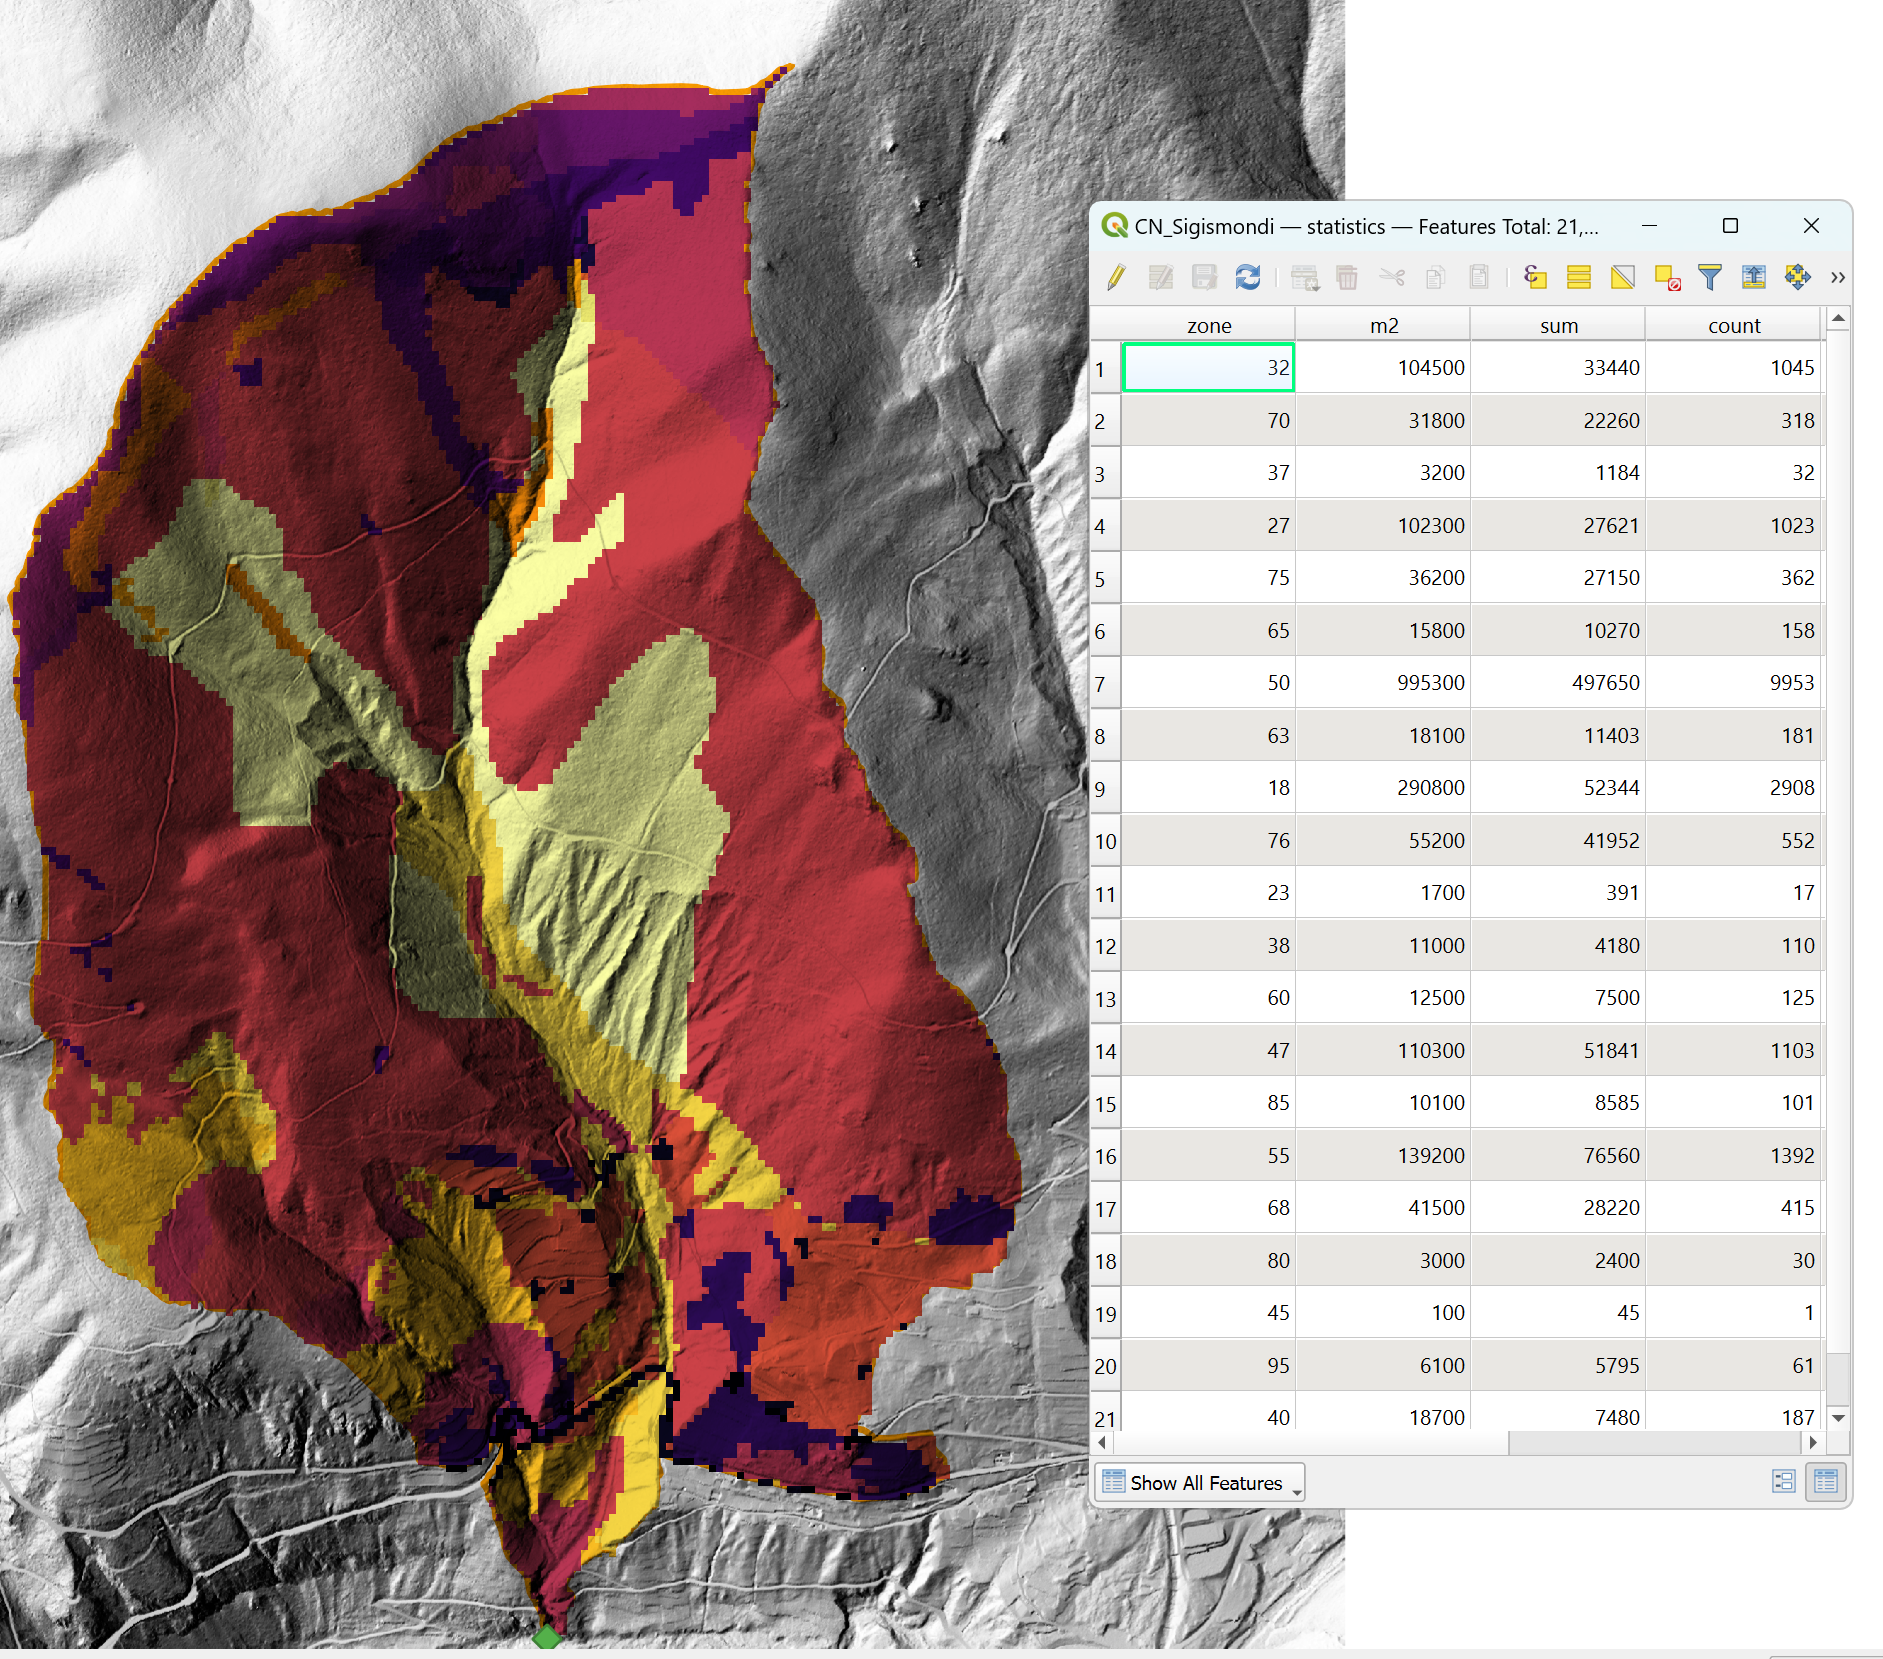
\includegraphics[scale=0.25]{immagini/qgis_cn.png}
    \caption{Attribuzione ad ogni cella del file raster del proprio parametro CN.}
    \label{qgis_cn}
\end{figure}

Ad ogni cella del file raster, di 10 metri di lato, sono state associati dei precisi valori di CN, a seconda del relativo suolo e soprassuolo. Successivamente, è stato calcolato il CN soppesato per la relativa area; tali valori sono stati sommati ed infine rapportati con l'area totale del bacino.
\begin{table}[H] \centering
    \caption{\textcolor{red}{Aree del bacino con valori di CN uguali.}}
    \begin{tabular}{ccc}
        \toprule
    \multicolumn{3}{c}{\textbf{Rio Sigismondi}}  \\
    Valore CN & Superficie ($km^2$) & $CN \cdot Ai$   \\
    \midrule
    18                 & 0.29                           & 5.2344            \\
    23                 & 0.00                           & 0.0391            \\
    27                 & 0.10                           & 2.7621            \\
    32                 & 0.10                           & 3.344             \\
    37                 & 0.00                           & 0.1184            \\
    38                 & 0.01                           & 0.418             \\
    40                 & 0.02                           & 0.748             \\
    45                 & 0.00                           & 0.0045            \\
    47                 & 0.11                           & 5.1841            \\
    50                 & 1.00                           & 49.765            \\
    55                 & 0.14                           & 7.656             \\
    60                 & 0.01                           & 0.75              \\
    63                 & 0.02                           & 1.1403            \\
    65                 & 0.02                           & 1.027             \\
    68                 & 0.04                           & 2.822             \\
    70                 & 0.03                           & 2.226             \\
    75                 & 0.04                           & 2.715             \\
    76                 & 0.06                           & 4.1952            \\
    80                 & 0.00                           & 0.24              \\
    85                 & 0.01                           & 0.8585            \\
    95                 & 0.01                           & 0.5795            \\
    \midrule
          & Area del Bacino ($km^2$) & CN medio\\
   & 2.00740               & 45.74   \\
   \bottomrule
    \end{tabular}
    \end{table}

Essendo il CN (II) pari a 45,74, l'applicazione della formula \ref{amcIII} permette di ricavare il CN(III), che è pari a 65.98.\\
La quantità che porta il terreno a saturazione è calcolabile con la formula \ref{parametro_S}, e con il coefficiente CN(III): in questo caso è pari a 130.98 mm.\\
Successivamente, avendo il valore dello storage S, è possibile calcolare la perdita iniziale di acqua ($I_a$), che varia da 0 a $0.2\cdot S$; riguarda tutto il volume di pioggia intercettata dalla vegetazione, o dalle cavità nel terreno, che non si infiltra e che non diventa deflusso. Al fine di creare una condizione cautelativa, si è scelto di applicare il coefficiente 0.05, in modo che la perdita iniziale diventi 6.55 mm.

\subsection{Calcolo del coefficiente di deflusso del bacino}
In modo similare al metodo precedente, il coefficiente di deflusso indica quanto del volume di pioggia diventa deflusso.\\
Al contrario del metodo CN, che considera la quantità d'acqua infiltrata, defluita o persa inizialmente, questo coefficiente indica solamente il volume di runoff misurato alla sezione di chiusura del bacino.\\
Ad ogni combinazione di suolo e soprassuolo viene associato un valore, da 0 ad 1; maggiore è il numero e maggiore è la quantità di precipitazione che si trasforma in pioggia efficace (deflusso).\\
Per esempio, le aree di territorio asfaltate (come per esempio strade) hanno un coefficiente di deflusso pari a 0.95, mentre i prati stabili ne hanno uno di 0.17.\\
Anche per questo metodo, è possibile calcolare il coefficiente di deflusso totale del bacino, avendo quelli delle singole aree, mediante la formula:
\begin{equation}
    c_{tot}=\frac{\sum c \cdot A_i}{A_{tot}}
\end{equation}
Come svolto in precedenza, è possibile conoscere i coefficienti di deflusso delle aree del bacino mediante il file raster reso disponibile dalla Provincia Autonoma di Trento, al seguente link: \url{https://siat.provincia.tn.it/geonetwork/srv/ita/catalog.search#/home}.
\begin{figure}[H]  \centering
    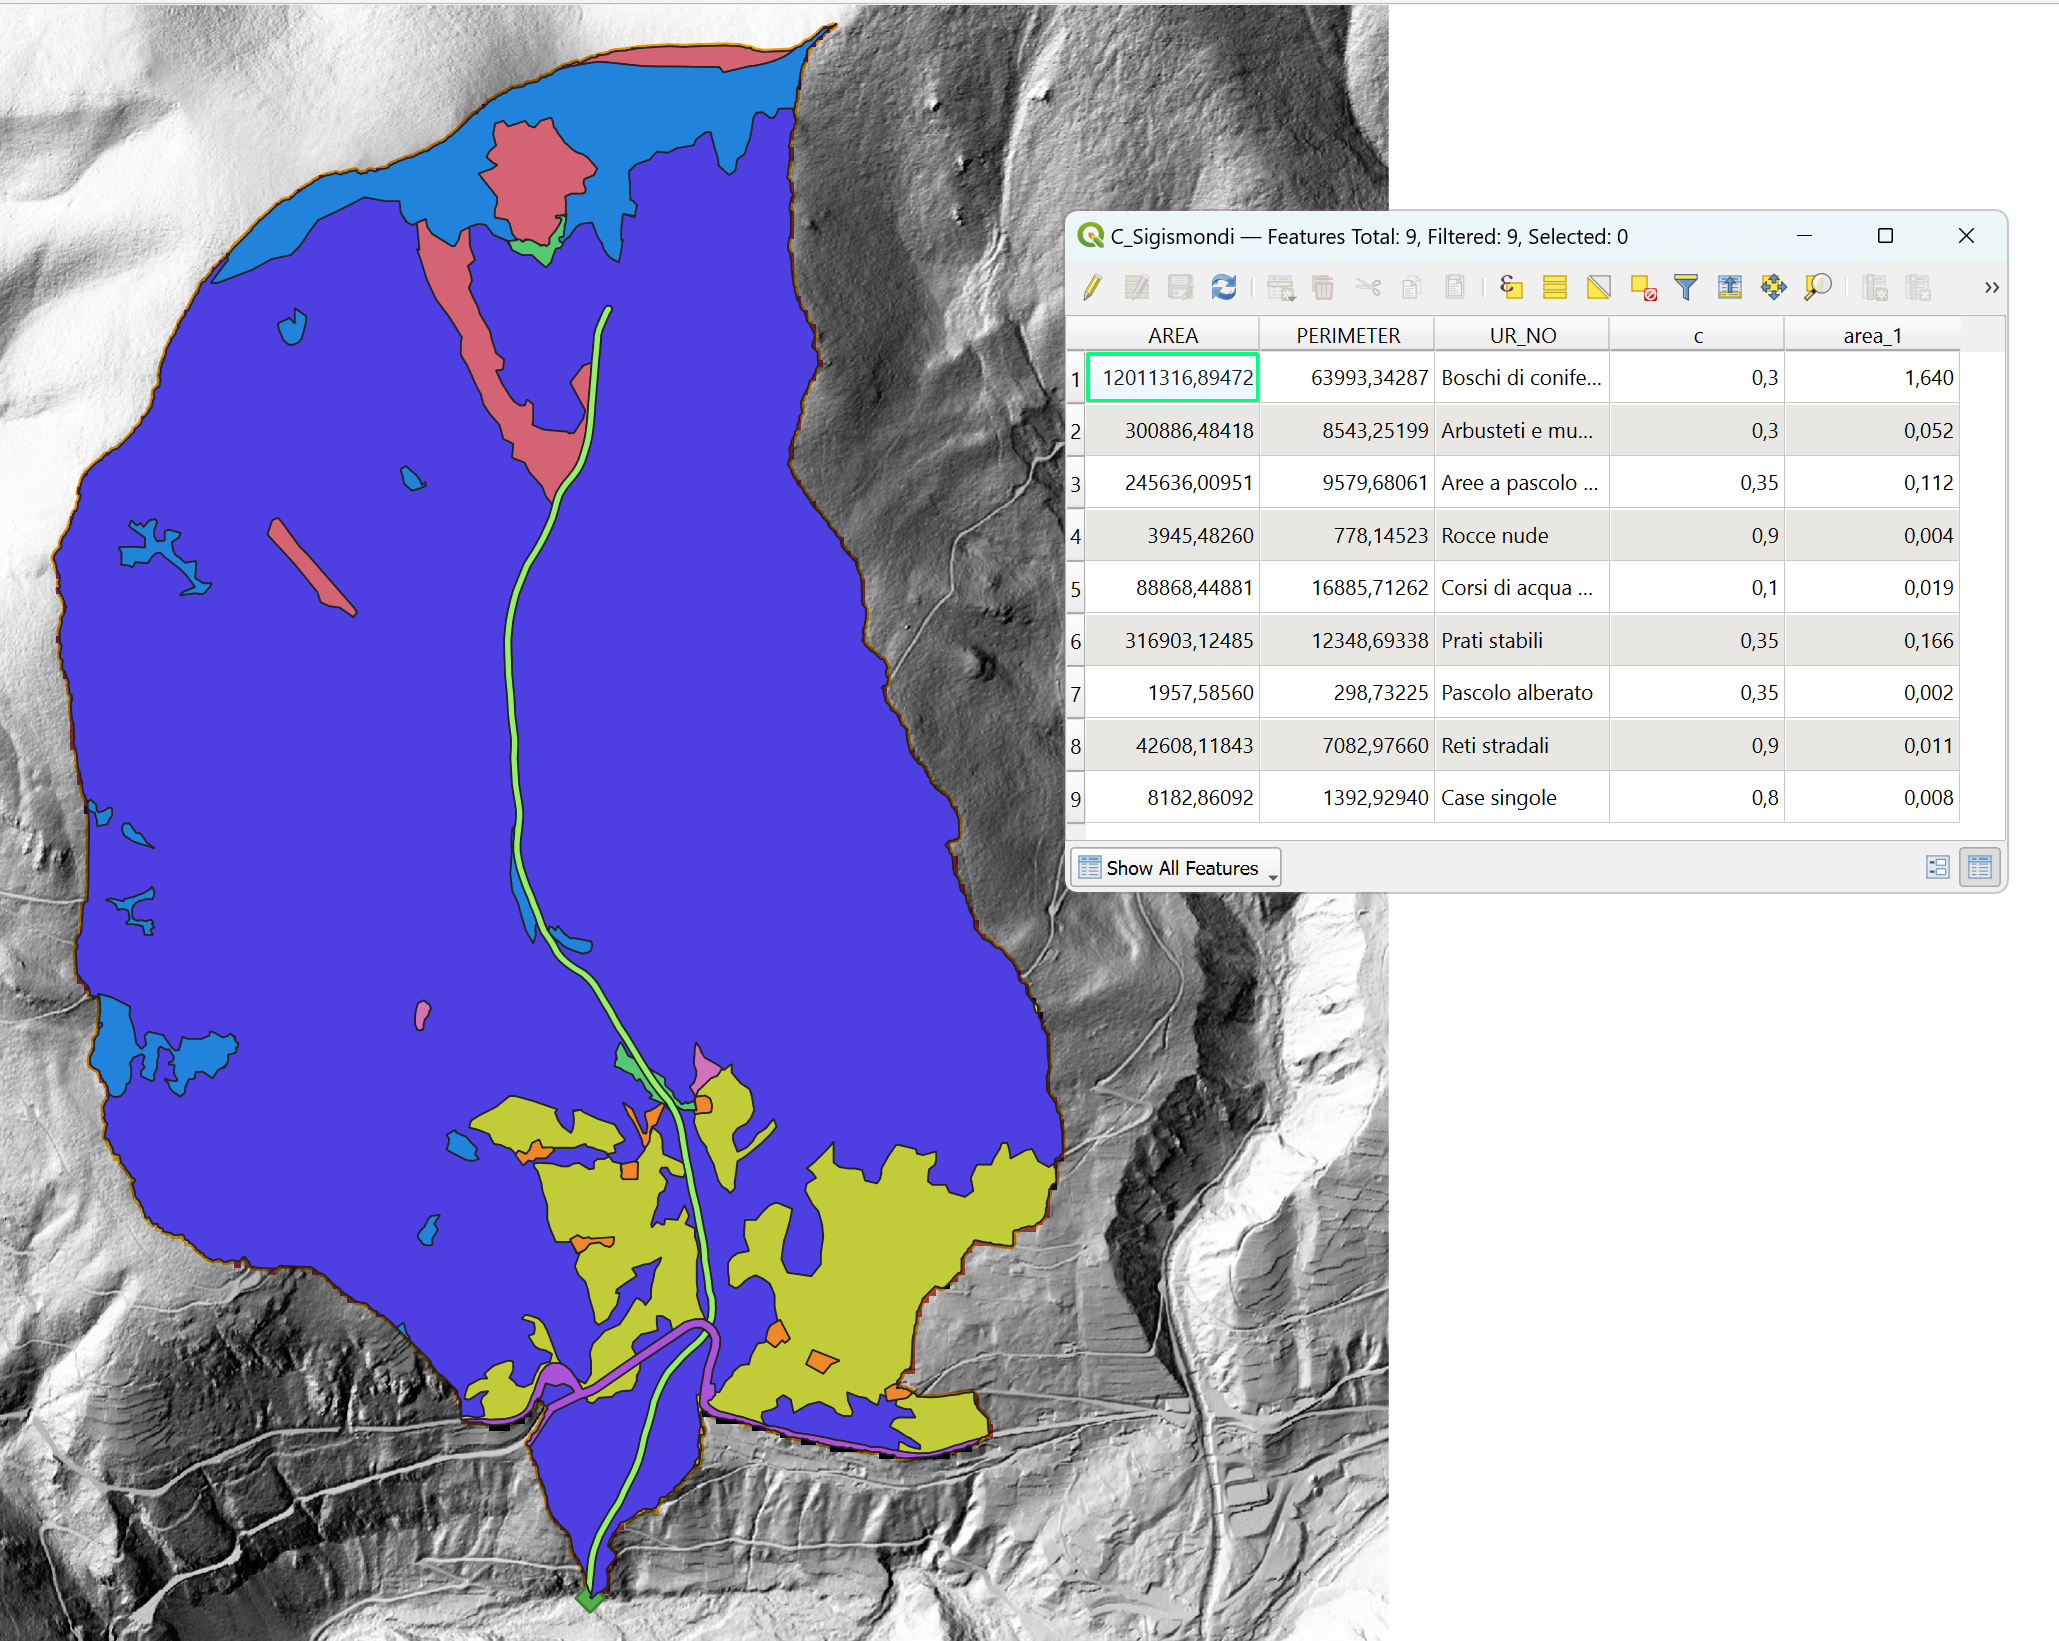
\includegraphics[scale=0.25]{immagini/qgis_c.png}
    \caption{Attribuzione ad ogni cella del file raster del proprio coefficiente di deflusso.}
    \label{qgis_c}
\end{figure}
Mediante il software Qgis è possibile estrarre i relativi valori:

\begin{table}[H] \centering
    \caption{\textcolor{red}{Aree del bacino con valori di coefficienti di deflusso uguali.}}
    \begin{tabular}{cccc}
    \toprule
    \multicolumn{4}{c}{\textbf{Rio Sigismondi}}\\
    \midrule
    Uso del suolo & Superficie ($km^2$)      & Valore C           & $C\cdot Ai$    \\
    & \textbf{}   & \textit{\textbf{}} &         \\
    Boschi di conifere                               & 1.64                  & 0.3                & 0.492   \\
    Arbusteti e mugheti                              & 0.05                  & 0.3                & 0.0156  \\
    Aree a pascolo naturale e praterie di alta quota & 0.11                  & 0.35               & 0.0392  \\
    Rocce nude                                       & 0.00                  & 0.9                & 0.0036  \\
    Corsi di acqua naturale                          & 0.02                  & 0.1                & 0.0019  \\
    Prati stabili                                    & 0.17                  & 0.35               & 0.0581  \\
    Pascolo alberato                                 & 0.00                  & 0.35               & 0.0007  \\
    Reti stradali                                    & 0.01                  & 0.9                & 0.0099  \\
    Case singole                                     & 0.01                  & 0.8                & 0.0064  \\
    \midrule
& Area del Bacino (km2) &  & C medio \\
  & 2.01400               &                    & 0.31 \\
  \bottomrule  
    \end{tabular}
    \end{table}

Come verrà ricordato anche successivamente, è generalmente preferito l'utilizzo del metodo SCS-CN, poiché non considera solamente il deflusso della pioggia arrivata al suolo, ma attribuisce valore anche a quella persa inizialmente o infiltrata.    

\subsection{Calcolo della pioggia efficace}
Al fine di conoscere le quantità di pioggia che si trasformano in deflusso (pioggia efficace), che vengono intercettate o che vengono assorbite, viene applicata la formula 
\begin{equation}
P_e = \frac{(P-I_a)^2}{P-I_a+S} 
\label{eq_PE}
\end{equation}
che deriva dalle seguenti:
\begin{figure}[H]
\begin{equation}
    \frac{P_e}{P-I_a} = \frac{F_a}{S} 
\end{equation}
\caption*{Relazione empirica che lega le diverse componenti dell'acqua meteorica in arrivo.}
\end{figure}
\begin{figure}[H]
\begin{equation}
    P= P_e + I_a + F_a     
\end{equation}
\caption*{Equazione di continuità.}
\end{figure}

Dovendo, per questa relazione, calcolare la pioggia efficace per diversi tempi di ritorno, è necessario tenere presente la tabella con i parametri della LSPP \ref{parametri_LSPP}, e dei parametri per la funzione del calcolo della $P_e$:
\begin{table}[H] \centering
    \caption{\textcolor{red}{Parametri sull'utilizzo del suolo e del soprassuolo del bacino.}}
    \begin{tabular}{cccc}
    \toprule   
  CN (II)  & CN (III)  & S (mm) & $I_a$ (mm)  \\
  45.74  &      65.98       & 130.98  & 6.55 \\
  \bottomrule  
    \end{tabular}
    \end{table}

Volendo considerare la precipitazione critica, ovvero dove la durata di pioggia eguaglia il tempo di corrivazione del bacino, l'evento pluviometrico deve durare 1.39 ore, come calcolato precedentemente mediante il metodo cinematico.\\
Il calcolo della pioggia critica avviene mediante la sostituzione dei parametri calcolati della LSPP, nella formula $h=a\cdot t^n$.\\
Infine, la pioggia efficace critica $Pe_{cr}$ si ricava applicando la formula \ref{eq_PE}.
    			
\begin{table}[H] \centering
    \caption{\textcolor{red}{Tabella contente i parametri necessari al calcolo della pioggia efficace critica.}}
    \begin{tabular}{cccc}
        \toprule
        & $T_c$ (ore) & $P_{cr}$  & $Pe_{cr}$ (mm) \\
        \midrule
        Tr=2 anni   & 1.39     & 26.50 & 2.64       \\
        Tr=5 anni   & 1.39     & 33.64 & 4.64       \\
        Tr=30 anni  & 1.39     & 45.50 & 8.93       \\
        Tr=50 anni  & 1.39     & 48.76 & 10.29      \\
        Tr=100 anni & 1.39     & 53.15 & 12.23      \\
        Tr=200 anni & 1.39     & 57.53 & 14.28      \\
        \bottomrule
\end{tabular}
\label{parametri_pioggia_efficace}
\end{table}
Ovviamente, all'aumentare del tempo di ritorno dell'evento, oltre a crescere l'altezza di pioggia, aumenta anche la quantità di acqua che diventa deflusso.

\subsection{Calcolo della portata al colmo}
Al fine di dimensionare correttamente una qualsiasi opera idraulica, è necessario conoscere il picco della portata di deflusso. In tal modo è possibile adattare qualsiasi struttura in modo che riesca a contenere la maggior portata di fluido in movimento, pur se interessa un arco di tempo piccolo.
Esistono diversi metodi per calcolare il picco di portata, in questa relazione ne verranno utilizzati tre, in modo da analizzare le differenze di applicazione e lo scostamento dei risultati.
\subsubsection{Metodo razionale}
Questo metodo è affidabile per bacini di ridotta superficie (inferiore ai 2-3 $km^2$), mentre è applicabile anche a bacini più grandi (fino a 50 $km^2$).\\
Al fine di applicare questo metodo, è necessario imporre alcune ipotesi:
\begin{itemize}
    \item la pioggia è di intensità costante e distribuita uniformemente sul bacino;
    \item la durata critica della precipitazione è pari al tempo di corrivazione $T_c$ del bacino. Se, a parità di altezza, la durata di pioggia fosse maggiore al $t_c$, l'intensità di precipitazione sarebbe minore. Infine, se la durata di pioggia fosse minore al $t_c$, non tutto il bacino sarebbe contribuente al medesimo istante;
    \item l'idrogramma di piena è di forma triangolare isoscele e di durata pari a $2 \cdot T_c$
\end{itemize}
Considerando le ipotesi appena elencate, la dimostrazione del metodo razionale può avvenire utilizzando la geometria.\\
Considerando che il volume efficace d'acqua affluito equivale al volume defluito, risulta vera l'uguaglianza che $P_e \cdot A =$ area dell'idrogramma di piena. Quest'ultima può anche essere vista come l'area di un triangolo, con base pari a 2$T_c$ ed altezza pari al deflusso di picco: $V = \frac{2 \cdot T_c Q_t}{2} \rightarrow T_c \cdot Q_t$.\\
Unendo le formule, risulta che $Q_t \cdot T_c = P_e \cdot A$ ed infine $Q_t \frac{P_e \cdot A}{T_c}$.

\begin{figure}[H]  \centering
    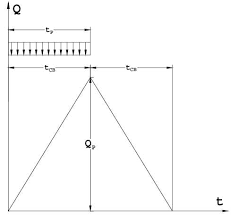
\includegraphics[scale=0.75]{immagini/metodo_razionale_deflusso.png}
    \caption{Rappresentazione minimale del metodo razionale per il calcolo del deflusso alla sezione di chiusura.}
    \label{metodo_razionale_deflusso}
\end{figure}

Nel caso in cui si utilizzassero le seguenti unità di misura:
\begin{itemize}
    \item $Q_t$ = $\frac{m^3}{s}$;
    \item $T_c$ = ore;
    \item $P_e$ = mm;
    \item A = $km^2$;
\end{itemize}
è possibile trasformare la formula del picco in:
\begin{equation}
    Q_t = \frac{P_e \cdot A}{3.6 \cdot T_c} + Q_{base}
    \label{picco_deflusso_Qt}
\end{equation}
Generalmente, la portata di base $Q_{base}$ viene considerata pari al 10\% della portata di picco.

\subsubsection{Metodo razionale utilizzando il CN}
Il calcolo della portata di picco di deflusso, utilizzando il metodo razionale ed il valore CN medio, avviene applicando la formula del calcolo di picco \ref{picco_deflusso_Qt} ai valori di pioggia efficace \ref{parametri_pioggia_efficace}.

\begin{table}[H] \centering
    \caption{\textcolor{red}{Risultati delle portate di picco, di base e totali per diversi tempi di ritorno.}}
    \begin{tabular}{ccccccc}
    \toprule
         & \multicolumn{2}{c}{Qt} & \multicolumn{2}{c}{Qbase} & \multicolumn{2}{c}{Qt+Qbase} \\
    \midrule
    Q2   & 1.06       & m3/s      & 0.11        & m3/s        & 1.17          & m3/s         \\
    Q5   & 1.87       & m3/s      & 0.19        & m3/s        & 2.05          & m3/s         \\
    Q30  & 3.59       & m3/s      & 0.36        & m3/s        & 3.95          & m3/s         \\
    Q50  & 4.13       & m3/s      & 0.41        & m3/s        & 4.55          & m3/s         \\
    Q100 & 4.91       & m3/s      & 0.49        & m3/s        & 5.40          & m3/s         \\
    Q200 & 5.74       & m3/s      & 0.57        & m3/s        & 6.31          & m3/s  \\
    \bottomrule      
    \end{tabular}
    \end{table}

Al fine di vedere graficamente come varia la portata alla sezione di chiusura, è necessario suddividere il deflusso per i tre istanti di maggior interesse, ovvero all'inizio e fine (ovvero portata di base) ed a metà evento (ovvero al picco). Per fare ciò, si crea una tabella che suddivide gli istanti, da cui è possibile creare un grafico a linee.

\begin{table}[H] \centering
    \caption{\textcolor{red}{Portate di deflusso alla sezione di chiusura, a seconda dell'attimo considerato.}}
    \begin{tabular}{ccccccc}
        \toprule
    tempo & \multicolumn{6}{c}{Qt+Qbase}           \\
    \midrule
& Tr=2anni & Tr=5anni & Tr=30anni & Tr=50anni & Tr=100anni & Tr=200anni \\
0 & 0.11  & 0.19     & 0.36      & 0.41      & 0.49       & 0.57       \\ 1.39 & 1.17  & 2.05  & 3.95      & 4.55      & 5.40       & 6.31       \\
2.78 & 0.11 & 0.19     & 0.36      & 0.41      & 0.49       & 0.57 \\
\bottomrule     
    \end{tabular}
    \end{table}

\begin{figure}[H]  \centering
        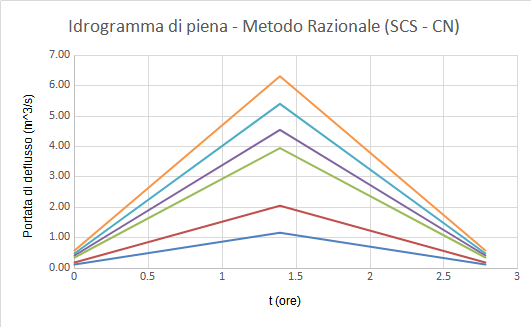
\includegraphics[scale=0.75]{immagini/metodo_razionale_scs_cn.png}
        \caption{Rappresentazione grafica dell'idrogramma di piena di deflusso, mediante il metodo razionale ed attraverso SCS-CN.}
        \label{metodo_razionale_scs_cn}
\end{figure}

\subsubsection{Metodo razionale utilizzando il coefficiente di deflusso}
In modo analogo al precedente procedimento, in questo paragrafo si andrà a calcolare il picco di deflusso del bacino, andando però a considerare il coefficiente di deflusso (e non il parametro CN).\\
Avendo già riportato i passaggi precedentemente, verranno solamente riportati i valori intermedi ed i risultati finali.
\begin{table}[H] \centering
    \caption{\textcolor{red}{Calcolo della pioggia efficace, mediante l'utilizzo del coefficiente di deflusso, calcolato in precedenza}}
    \begin{tabular}{cccc}
        \toprule
                & Tc (ore) & P cr  & Pe cr (mm) \\
        \midrule
    Tr=2 anni   & 1.39     & 26.50 & 2.64       \\
    Tr=5 anni   & 1.39     & 33.64 & 4.64       \\
    Tr=30 anni  & 1.39     & 45.50 & 8.93       \\
    Tr=50 anni  & 1.39     & 48.76 & 10.29      \\
    Tr=100 anni & 1.39     & 53.15 & 12.23      \\
    Tr=200 anni & 1.39     & 57.53 & 14.28      \\
    \bottomrule
    \end{tabular}
    \end{table}

\begin{table}[H] \centering
        \caption{\textcolor{red}{Risultati delle portate di picco, di base e totali per diversi tempi di ritorno.}}
        \begin{tabular}{ccccccc}
            \toprule
        & \multicolumn{2}{c}{Qt} & \multicolumn{2}{c}{Qbase} & \multicolumn{2}{c}{Qt+Qbase} \\
        \midrule
        Q2   & 1.06       & m3/s      & 0.11        & m3/s        & 1.17          & m3/s         \\
        Q5   & 1.87       & m3/s      & 0.19        & m3/s        & 2.05          & m3/s         \\
        Q30  & 3.59       & m3/s      & 0.36        & m3/s        & 3.95          & m3/s         \\
        Q50  & 4.13       & m3/s      & 0.41        & m3/s        & 4.55          & m3/s         \\
        Q100 & 4.91       & m3/s      & 0.49        & m3/s        & 5.40          & m3/s         \\
        Q200 & 5.74       & m3/s      & 0.57        & m3/s        & 6.31          & m3/s    \\
        \bottomrule    
        \end{tabular}
\end{table}

\begin{table}[H] \centering
    \caption{\textcolor{red}{Portate di deflusso alla sezione di chiusura, a seconda dell'attimo considerato.}}
    \begin{tabular}{ccccccc}
        \toprule
    tempo & \multicolumn{6}{c}{Qt+Qbase}    \\
    \midrule
& Tr=2anni & Tr=5anni & Tr=30anni & Tr=50anni & Tr=100anni & Tr=200anni \\
    0                      & 0.11     & 0.19     & 0.36      & 0.41      & 0.49       & 0.57       \\
    1.39                   & 1.17     & 2.05     & 3.95      & 4.55      & 5.40       & 6.31       \\
    2.78                   & 0.11     & 0.19     & 0.36      & 0.41      & 0.49       & 0.57 \\
    \bottomrule     
    \end{tabular}
\end{table}

\begin{figure}[H]  \centering
    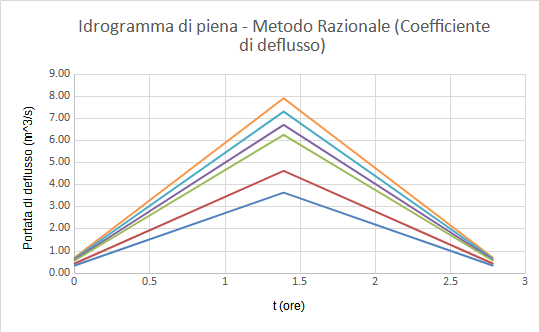
\includegraphics[scale=0.75]{immagini/metodo_razionale_coefficiente_deflusso.png}
    \caption{Rappresentazione grafica dell'idrogramma di piena di deflusso, mediante il metodo razionale ed attraverso il coefficiente di deflusso.}
    \label{metodo_razionale_coefficiete_deflusso}
\end{figure}

\subsubsection{Confronto tra il metodo razionale mediante SCS-CN ed il coeff. di deflusso}
Com'è possibile notare negli idrogrammi precedenti, e nell'immagine successiva, il metodo razionale calcolato mediante il coefficiente tende a generare una curva di deflusso maggiore rispetto a quella che utilizza il CN.

\begin{figure}[H]  \centering
    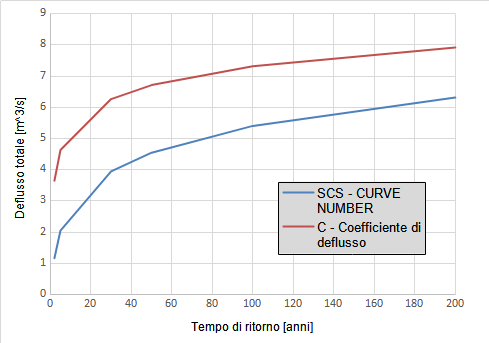
\includegraphics[scale=0.75]{immagini/metodo_razionale_cn_c.png}
    \caption{Andamenti delle portate uscenti, secondo il metodo SCS-CN e secondo il coefficiente di deflusso.}
    \label{metodo_razionale_cn_c}
\end{figure}
In entrambi i casi, all'aumentare del tempo di ritorno dell'evento, il deflusso aumenta in maniera meno che proporzionale.

\subsubsection{Metodo empirico - Forti (II)}
Per il campo di applicazione interno al territorio italiano, in letteratura scientifica sono disponibili alcune formule empiriche per il calcolo della portata unitaria di picco del bacino ($q$).\\
Per il solo fine di esempio, si è deciso di applicare la formula di Forti (II):
\begin{equation}
    q = 2.35 \cdot \frac{500}{A+125}+0.5
\end{equation}
Questo metodo prevede che l'evento pluviometrico che genera il deflusso abbia apportato al suolo un'altezza di precipitazione di 200-250 mm, per la durata di 24 ore.\\
Essendo che la superficie del bacino in analisi è di 2.01 $km^2$, l'applicazione della precedente formula restituisce un valore di portata unitaria pari a 9.75 $\frac{m^3}{s \cdot km^2}$; di conseguenza, la portata di picco Q del bacino è pari a 19.60 $\frac{m^3}{s}$.\\
Confrontando tale valore con quelli precedenti, ne risulta che quello calcolato con il metodo empirico tende a sovrastimare eccessivamente l'evento idraulico uscente dal bacino.

\subsection{Studio del deflusso con tempo di pioggia superiore a quello di corrivazione}
E' raro che la durata dell'evento di pioggia sia uguale al tempo di corrivazione del bacino; generalmente, la durata di pioggia è ben superiore al tempo di risposta totale del bacino. Questa condizione comporta due fenomeni: un minore picco di deflusso, ma un maggior volume di acqua uscente dalla sezione di chiusura.
Per valutare come si comporta il bacino in risposta a precipitazioni di durate superiori a quella di corrivazione, sono stati ripetuti i calcoli del metodo razionale, a seconda del tempo di ritorno e del tempo di pioggia.\\
Per valori sempre maggiori della durata di pioggia, sono stati ripetuti i calcoli inerenti alla pioggia efficace, alla portata di picco ed al volume totale.
\begin{figure}[H]  \centering
    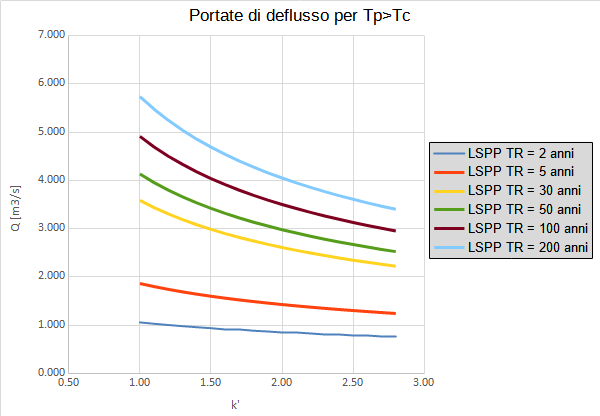
\includegraphics[scale=0.75]{immagini/deflusso_tp_tc.png}
    \caption{Andamento del deflusso per ogni tempo di ritorno.}
    \label{metodo_razionale_cn_c}
\end{figure}
Per tempi di ritorno relativamente bassi, la riduzione del picco della portata di deflusso è più attenuata rispetto a quella che si noterebbe per tempi di ritorno superiori.